% -*- latex -*-

\documentclass[twocolumn]{article}

\usepackage[usenames]{color}
\definecolor{Red}{rgb}{1,0,0}
\newcommand{\sticky}[1]{\textcolor{Red}{[#1]}}

\usepackage{graphicx}
\usepackage{varioref}
\usepackage{hyperref}

\title{From Cluster to Wall with VTK}
\author{Kenneth~Moreland}

\begin{document}

\maketitle

\begin{abstract}
  This paper describes new parallel rendering component for VTK, the
  Visualization Toolkit.  The parallel rendering unit allows for vast
  quantities of geometry to be rendered on cluster computers.  Furthermore,
  the geometry may be displayed on tiled displays at full or reduced
  resolution.  We have demonstrated an interactive VTK application
  processing an isosurface consisting of nearling half a billion triangles
  and displaying on a power wall with a total resolution of 60 Mega-pixels
  ($60*2^{20}$ pixels) in an interactive application.  We also demonstrate
  an interactive VTK application displaying the same geometry on a desktop
  connected to the cluster via a TCP/IP socket over 100BASE-T Ethernet.
\end{abstract}

\section{Introduction}
\label{sec:introduction}

``That's great.  How can I use it?''  This is the question our
visualization research team is faced with whenever we present a promising
new tool to our analysts.  Until recently, our best solution was to wrap
the tool in its own user interface.  This proliferation of visualization
tools wastes human resources on many fronts.  It requires our researchers
to design, build, and maintain user interfaces for their tools.  Since our
visualization researchers are often neither motivated nor experieced at
designing user interfaces, the tool interfaces are often ill-conceived,
rarely consistent, and never tightly coupled.  Analysts are forced to learn
a wide variety of interfaces for the tools they wish to use, if they are
aware of the tools' existance at all.  Often this results in tools being
unused.

To alleviate these problems, we have chosen to leverage VTK, the
Visualization Toolkit \cite{Schroeder98}.  VTK is an open-source API
containing a comprehensive suite of visualization tools.  More importantly,
VTK incorporates an extendible component-based architecture.  Our new
approach to delivering visualization tools is to wrap these tools into VTK
components and store these components in a common component library.  This
should allow each tool to work together with current and future tools under
the same, consistent user interface.  All three national labs, Sandia, Las
Alamos, and Lawrence Livermore \sticky{Am I right in saying \emph{the}
national labs, or is there some other classification?  Are they the three
DOE labs?}, have agreed to make VTK the R\&D platform for visualization.

Our visualization needs put a large strain on VTK.  ASCI routinely creates
simulations on the order of 50 million cells \cite{Heermann99}, and it is
predicted that by 2004 ASCI will routinely create 250 million cell
simulations requiring up to a petabyte of storage \cite{Smith98}.  The
processing of such data is well beyond the capabilities of a standard
workstation.  Our most cost effective means for handling this data in a
timely manner is the use of commodity cluster computers running distributed
memory algorithms.  The creation of such high fidelity models also
necessitates the use of high fidelity displays for visualization.  To
realize these high resolution displays we build ``power walls,'' projected
displays driven by tiled arrays of commodity projectors.  We require our
VTK applications to run interactively on clustered computers while either
driving a power wall or shipping images back to a remote computer for
desktop delivery.


\section{Previous Work}
\label{sec:previous_work}

Thanks to a recent collaberation between Kitware and the ASCI/VIEWS
program, VTK now supports parallel programming and can be run on cluster
computers \cite{Ahrens00}.  The parallel VTK libraries support several
parallel modes.  The mode we consern ourselves with in this paper is
``data'' parallelism in which the input data is split amongst processes,
the pieces are filtered and rendered independently, and then composited to
one image in the end.  This method allows us to make effective use of the
parallel and distributed nature of our clusters, but can break down if the
model pieces are too big to be processed by the available
resources\footnote{Ahrens et. al. \cite{Ahrens01} describe using VTK in a
streaming mode to perform out-of-core processing of data.}.

While parallel visualization and rendering are now supported by VTK,
display to a power wall and desktop delivery currently are not.  One
possible approach is to use Chromium \cite{Humphreys02}.  Chromium is
capable of replacing the OpenGL library loaded by an appliaction at
runtime, intercepting the stream of OpenGL commands, and performing several
altercations to it, including driving a power wall.  Unfortunately, an
OpenGL stream is inherently serial and must be issued from a single
process, which is a huge bottleneck when dealing with large amounts of
data.  Chromium also supports a parallel rendering mode, but an application
must be ``aware'' of Chromium to take advantage of this parallel rendering.
We are currently looking into ways to run VTK in a parallel Chromium
rendering environment.

Another power wall display solution available to us was ICE-T, the Image
Composite Engine for Tiles.  The ICE-T API is an implementation of the work
presented by Moreland, Wylie, and Pavlakos for efficiently performing
sort-last parallel rendering onto tile displays \cite{Moreland01}.  The
ICE-T methodology for rendering fits well with VTK's existing parallel
rendering paradigm.  We therefore implemented a new composite engine for
VTK using the ICE-T API, to be discussed in section
\ref{sec:tiled_display}.


\section{Desktop Delivery}
\label{sec:desktop_delivery}

Since we in no way expect each analyst to have a parallel cluster available
in his office, we find it important to provide the ability of remote
desktop delivery.  That is, we wish a user to be able to interactively
control a visualization job rendering on a cluster and display back to a
typical desktop machine connected via a modest LAN connection.

\begin{figure*}
  \begin{center}
    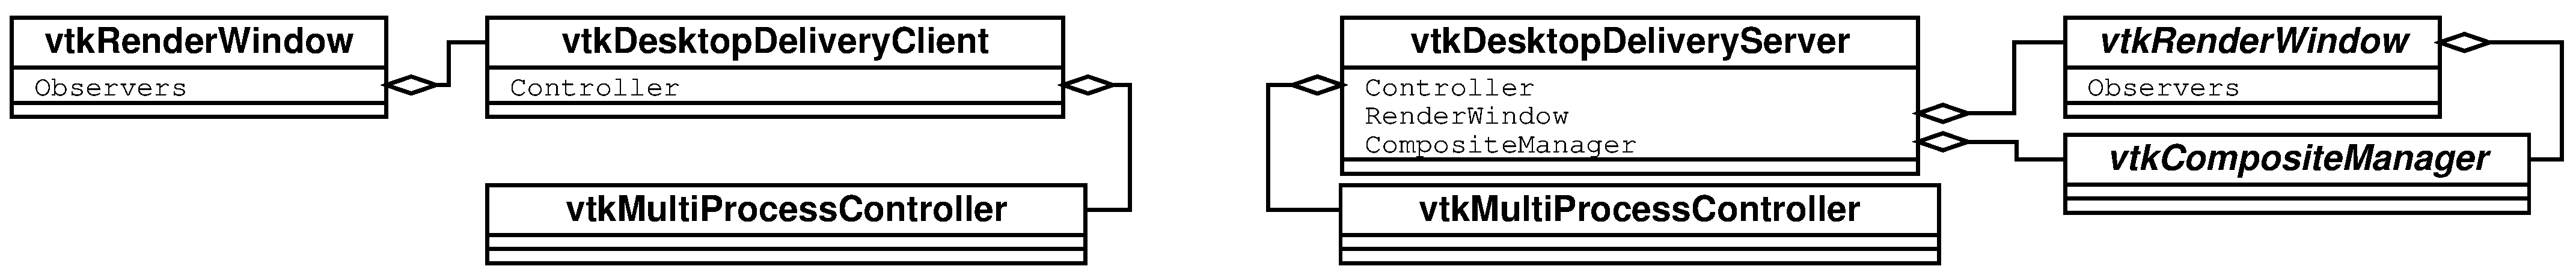
\includegraphics[scale=0.23]{images/DesktopDeliveryClasses}
  \end{center}
  \caption{UML diagrams for desktop delivery objects.}
  \label{fig:desktop_delivery_classes}
\end{figure*}

Figure \vref{fig:desktop_delivery_classes} shows the collaboration between
the desktop delivery objects and other VTK components.  There are two
desktop delivery objects, one for the client, which accepts user input and
displays rendered images, and one for the server, which performs the
visualization processing and rendering.  The two objects are connected
together with a pair of vtkMultiProcessController objects.
vtkMultiProcessController is an abstract interface to parallel process
controll and communication.  The desktop delivery objects expect the proces
controller to controll exactly two objects with client and server in
opposite processes.  The controller is typically implemented with a socket,
but does not have to be.

\begin{figure}[ht]
  \begin{center}
    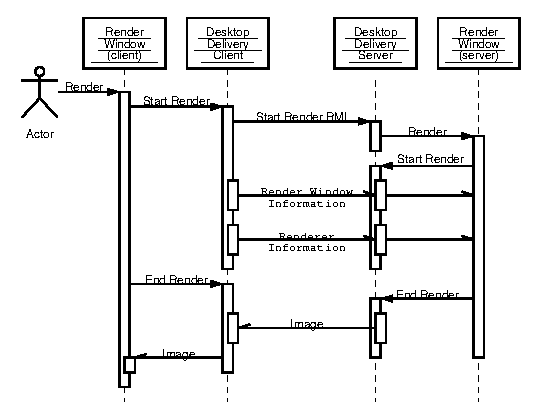
\includegraphics[scale=0.23]{images/DesktopDeliveryInteraction}
    \caption{Interactions during rendering with desktop delivery.}
    \label{fig:desktop_delivery_interaction}
  \end{center}
\end{figure}

The desktop delivery client object attaches itself as an observer to a
render window.  When a render event occurs, the desktop delivery client
object sends a render request to the server, waits for an image to come
back, and pasts the image to the window.  Figure
\vref{fig:desktop_delivery_interaction} shows the details of this process.

Because the desktop delivery server was designed to enable delivery from
clusters, it can optionally work with a vtkCompositeManager object, which
is the object VTK uses to perform sort-last parallel rendering.  The
desktop delivery server object uses the composite manager to compute the
complete object bounds, get timing statistics, and otherwise controll the
parallel rendering process.

We also want the remote rendering's interactivity to be resilient to
network speeds and rendering image size.  This is done with a reduction
factor option, a concept borrowed from the vtkCompositeManager class.  This
option reduces the width and height of the rendered image by the factor
given and then expands the image with pixel replication on the client side.
The reduced image size can save time in server client transfer times as
well as composite times in parallel applications.  In addition,
vtkDesktopDeliveryClient has the capability to adjust the reduction factor
based on timings of the previous run and the desired rendering rate set in
the render window.


\section{Tiled Display}
\label{sec:tiled_display}

\begin{figure*}
  \begin{center}
    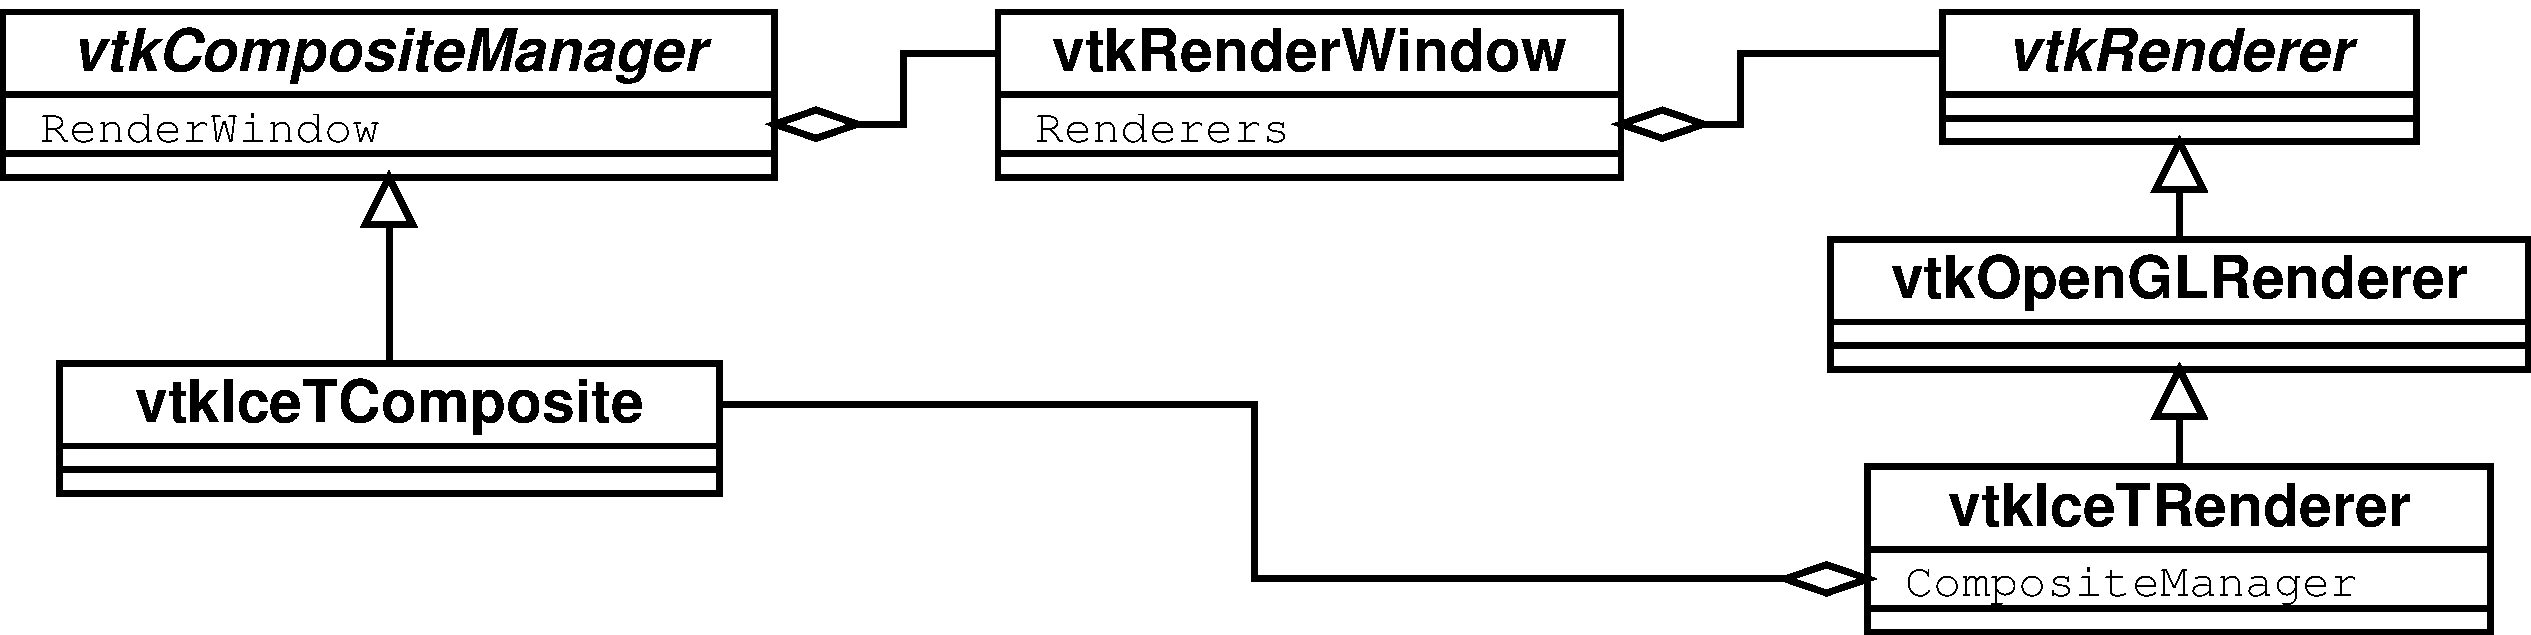
\includegraphics[scale=0.23]{images/IceTCompositeClasses}
  \end{center}
  \caption{UML diagram for tiled display compositing.}
  \label{fig:tiled_display_classes}
\end{figure*}

We also greatly desire to drive power walls in our parallel VTK
applications.  We did this by wrapping our ICE-T API in VTK objects.
First, we subclassed vtkCompositeManager to allow ICE-T to be a drop-in
replacement for any VTK compositor.  Unfortunatly, the ICE-T API exhibits
behavior that goes above and beyond what the VTK composite manager does.
In particular, because ICE-T generates images larger than the renderable
window of any given display, it must be able to render the same geometry
multiple times.  It must also be able to change the projection matrix
before each rendering.  This functionality was most easily introduced by
subclassing vtkOpenGLRenderer.  Under ``normal'' circumstances, the ICE-T
renderer behaves just like any other VTK renderer.  When used in
conjunction with the ICE-T composite manager, the ICE-T renderer invokes
the ICE-T API to manipulate projection matrices, render multiple viewing
frustums, and compose multiple images in parallel.  The ICE-T composite
manager does nothing but emit errors if not used with an ICE-T renderer.  A
diagram of these objects collaborate are shown in figure
\vref{fig:tiled_display_classes}.

Like the desktop delivery and other forms of the vtkCompositeManager
classes, the ICE-T composite manager also supports the idea of a reduction
factor.  Unlike the other reduction factor implementations, the ICE-T
composite manager does not reduce the size of the renderable window.
Recall that in a tiled display, the overall display size is larger than any
one image.  ICE-T uses an extension of the ``floating viewport'' described
in Moreland, Wylie, and Pavlakos \cite{Moreland01} to render images
spanning multiple tiles and therefore reduce the number of times the
geometry must be rendered.

Another important issue with rendering to tiled displays is providing an
interface with which users can interact.  The typical solution for VTK
applications using a composite manager such as ParaView is to place the
user interface at node 0 where the image is displayed \cite{Law01}.  This
is problematic with a tile display for several reasons.  The most
prevailing problem for us is the fact that, for security reasons, our
display wall and driving cluster are in different rooms, separated by a
bolted steel door.  Instead, our user interface resides on a ``steering
station,'' a separate PC located with the display and connected to the
cluster via a standard Ethernet connection.  Changes made in the user
interface running on the steering station are then propgated to the images
on the display wall.

It so happens that this exact functionality is already implemented by the
desktop delivery objects described in section \ref{sec:desktop_delivery}
except that images are displayed on the server rather than shipped back the
client.  Therefore, the desktop delivery server object has a flag to select
the display.  If displaying to the client, the behavior is as described in
section \ref{sec:desktop_delivery}.  If displaying to the server, the
render windows on the server side are never resized and images are not
transfered back to the client.  The client simply renders a very coarse
representation of the geometry, which is a bounding box by default.


\section{Discussion}
\label{sec:discussion}

With the introduction of the desktop delivery and ICE-T components into
VTK, we have shown that VTK is a viable framework for cluster-based
interactive applications that require remote display or display to
high-resolution power walls.  By using both the image-centric
level-of-detail provided by the reduction factor functionality of the
desktop delivery and ICE-T components in conjunction with the
geometry-centric level-of-detail directly provided by VTK, we can achieve
highly interactive rendering with almost any image transfer, compositing,
or rendering speeds.  \sticky{Some empirical evidence, i.e. with LLNL data,
would probably be good here.  But that would suggest adding more figures,
increasing the size of the paper, and making review and release harder.
Doing this probably depends on the forum.}

One drawback of the ICE-T composite objects is that they only work with
OpenGL rendering and MPI communications.  This is because, due to
historical reasons, the ICE-T API is dependent on the OpenGL and MPI APIs.
In retrospect, coupling the compositing API with any particular rendering
or communications API was not beneficial.  Nevertheless, OpenGL and MPI
remain the de facto \sticky{or should it be \emph{de facto}?} standards.


\section{Future Work}
\label{sec:future_work}

We have just begun to make a viable production-quality tool to run on our
clusters and display on our power walls.  There is much work to be done.

The use of ICE-T's image compositing to drive power walls has the advantage
of being resilient to changes in the input geometry size.  Unfortunately,
it also incurs a high overhead in each frame regardless of how little
geometry is to be rendered.  In situations like this, we could benefit
greatly from a sort-first architecture like the one implemented in the
``tilesort'' SPU of the Chromium system \cite{Humphreys02}.  It would be
interesting to directly compare the two approaches and find the cutoff in
geometry size, if any, where image compositing outweighs tile sorting.

Our desktop delivery objects allow for any type of interface to be built on
the client side.  However, we currently have not built a GUI cappable of
much more than simple navigation controls.  Ultimately, we would like a
fully featured visualization tool such as ParaView \cite{Law01} to be
presented at the desktop.

While the concept of a steering station (introduced in section
\ref{sec:tiled_display}) allows an arbitrarily complex user interface, it
can be less than ideal.  Often, we find the user jumping between the
steering station and the wall.  We would like to incorporate a hand-held
device that could move with the user and at least provide navigation
controls.


\bibliographystyle{plain}
\bibliography{vtkicet}

\end{document}
